\documentclass{standalone}
\usepackage{tikz}

\begin{document}
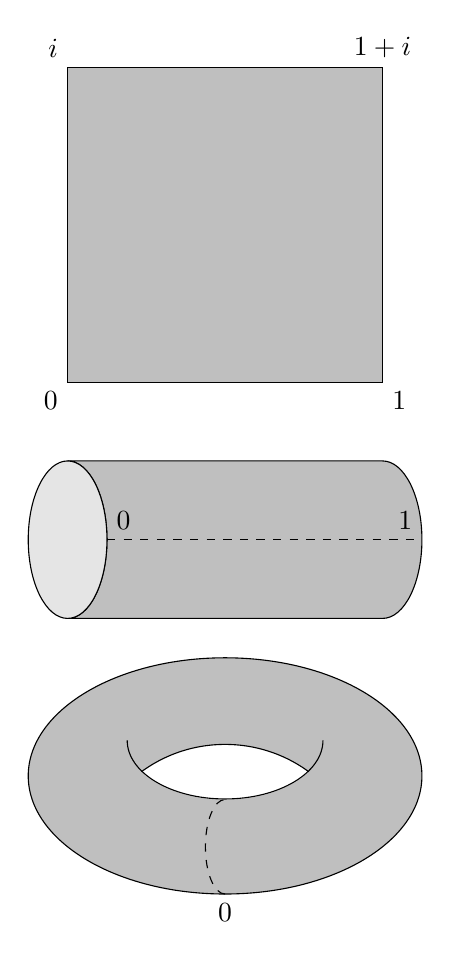
\begin{tikzpicture}
\filldraw[fill=gray!50] (0,0) -- (4,0) -- (4,4) -- (0,4) -- cycle;
\draw (0,0) node[anchor=north east]{$ 0 $};
\draw (4,0) node[anchor=north west]{$ 1 $};
\draw (4,4) node[anchor=south]{$ 1+i $};
\draw (0,4) node[anchor=south east]{$ i $};

\begin{scope}[yshift=-3cm]
	\filldraw[fill=gray!50] (0,0) arc[start angle=-90, end angle=90, x radius=0.5,
		y radius=1] -- (4,2) arc[start angle=90, end angle=-90, x radius=0.5, y
		radius=1] -- cycle;
	\filldraw[fill=gray!20] (0,1) ellipse (0.5 and 1);
	\draw[dashed] (0.5,1) -- (4.5, 1);
	\draw (0.5,1) node[anchor=south west]{$ 0 $};
	\draw (4.5,1) node[anchor=south east]{$ 1 $};
\end{scope}

\begin{scope}[yshift=-7cm]
	\filldraw[fill=gray!50] (2,2) ellipse (2.5 and 1.5);
	\begin{scope}
		\clip (2,2.45) ellipse (1.25 and 0.75);
		\filldraw[fill=white] (2,0.6) circle (1.8);
		\draw[thick] (0.75, 2.45) arc[start angle=180, end angle=360, x radius=1.25, y
			radius=0.75];
	\end{scope}
	\draw[dashed] (2,0.5) arc [start angle = 270, end angle=90, x radius=0.25, y
		radius=0.6];
	\draw (2,0.5) node[below]{$ 0 $};
\end{scope}
\end{tikzpicture}
\end{document}

